%%%%%%%%%%%%%%%%%%%%%%%%%%%%%%%%%%%%%%%%%%%%%%%%%%%%%%%%%%%%%%%%%%%%%%%%%%
%
% Plantilla para libro de texto de matemáticas.
%
% Esta plantilla ha sido desarrollada desde cero, pero utiliza algunas partes
% del código de la plantilla original utilizada en apuntesDGIIM
% (https://github.com/libreim/apuntesDGIIM), basada a su vez en las plantillas
% 'Short Sectioned Assignment' de Frits Wenneker (http://www.howtotex.com),
% 'Plantilla de Trabajo' de Mario Román y 'Plantilla básica de Latex en Español'
% de Andrés Herrera Poyatos (https://github.com/andreshp). También recoge
% ideas de la plantilla 'Multi-Purpose Large Font Title Page' de
% Frits Wenneker y Vel (vel@latextemplates.com).
%
% Licencia:	
% CC BY-NC-SA 4.0 (https://creativecommons.org/licenses/by-nc-sa/4.0/)
%
%%%%%%%%%%%%%%%%%%%%%%%%%%%%%%%%%%%%%%%%%%%%%%%%%%%%%%%%%%%%%%%%%%%%%%%%%

% ---------------------------------------------------------------------------
% CONFIGURACIÓN BÁSICA DEL DOCUMENTO
% ---------------------------------------------------------------------------

%\documentclass[11pt, a4paper, twoside]{article} % Usar para imprimir
\documentclass[10pt, a4paper]{article}

\linespread{1.3}            % Espaciado entre líneas.
\setlength\parindent{0pt}   % No indentar el texto por defecto.
\setlength\parskip{7pt}

% ---------------------------------------------------------------------------
% PAQUETES BÁSICOS
% ---------------------------------------------------------------------------

% IDIOMA
\usepackage[utf8]{inputenc}
\usepackage[spanish, es-tabla, es-lcroman, es-noquoting]{babel}
\usepackage[table,xcdraw]{xcolor}
\usepackage{longtable}
\usepackage{subfigure}

% MATEMÁTICAS
\usepackage{amsmath}    % Paquete básico de matemáticas
\usepackage{amsthm}     % Teoremas
\usepackage{mathrsfs}   % Fuente para ciertas letras utilizadas en matemáticas

% FUENTES
\usepackage{newpxtext, newpxmath}   % Fuente similar a Palatino
\usepackage{FiraSans}                 % Fuente sans serif
\usepackage[T1]{fontenc}
\usepackage[italic]{mathastext}     % Utiliza la fuente del documento
                                    % en los entornos matemáticos

% MÁRGENES
\usepackage[margin=2.5cm, top=3cm]{geometry}

% LISTAS
\usepackage{enumitem}       % Mejores listas
\setlist{leftmargin=.5in}   % Especifica la indentación para las listas.

% Listas ordenadas con números romanos (i), (ii), etc.
\newenvironment{nlist}
{\begin{enumerate}
    \renewcommand\labelenumi{(\emph{\roman{enumi})}}}
  {\end{enumerate}}

%  OTROS
\usepackage[hidelinks]{hyperref}   % Enlaces
\usepackage{graphicx}   % Permite incluir gráficos en el documento
\usepackage{relsize}

% LISTINGS
\usepackage{listings}
\usepackage{xcolor}     % Permite definir y utilizar colores
\usepackage{lipsum}
\usepackage{courier}

% Fijar tabla a posición
\usepackage{array}
\newcolumntype{L}[1]{>{\raggedright\let\newline\\\arraybackslash\hspace{0pt}}m{#1}}
\newcolumntype{C}[1]{>{\centering\let\newline\\\arraybackslash\hspace{0pt}}m{#1}}
\newcolumntype{R}[1]{>{\raggedleft\let\newline\\\arraybackslash\hspace{0pt}}m{#1}}

\setcounter{MaxMatrixCols}{20}

% Colores para los bloques de código
\definecolor{codegreen}{rgb}{0,0.6,0}
\definecolor{codegray}{rgb}{0.5,0.5,0.5}
\definecolor{codepurple}{rgb}{0.58,0,0.82}
\definecolor{backcolour}{rgb}{0.95,0.95,0.92}
\lstdefinestyle{mystyle}{
	backgroundcolor=\color{backcolour!70!white},   
	commentstyle=\color{codegreen},
	keywordstyle=\color{blue},
	numberstyle=\tiny\color{codegray},
	stringstyle=\color{codepurple},
	basicstyle=\footnotesize\ttfamily,
	breakatwhitespace=false,         
	breaklines=true,                 
	captionpos=b,                    
	keepspaces=true,                 
	numbers=left,                    
	numbersep=5pt,                  
	showspaces=false,                
	showstringspaces=false,
	showtabs=false,                  
	tabsize=4
}
\lstset{style=mystyle}

\usepackage{amsmath}
\usepackage{algorithm}


\usepackage[noend]{algpseudocode}

\makeatletter
\def\BState{\State\hskip-\ALG@thistlm}
\makeatother

%\lstset{basicstyle=\footnotesize\ttfamily,breaklines=true}
%\lstset{framextopmargin=50pt,frame=bottomline}
 
% ---------------------------------------------------------------------------
% COMANDOS PERSONALIZADOS
% ---------------------------------------------------------------------------

% \equalto
\newcommand{\verteq}{\rotatebox{90}{$\,=$}}
\newcommand{\equalto}[2]{\underset{\scriptstyle\overset{\mkern4mu\verteq}{#2}}{#1}}


% ---------------------------------------------------------------------------
% COLORES
% ---------------------------------------------------------------------------

\definecolor{50}{HTML}{E0F2F1}
\definecolor{100}{HTML}{B2DFDB}
\definecolor{200}{HTML}{80CBC4}
\definecolor{300}{HTML}{4DB6AC}
\definecolor{400}{HTML}{26A69A}
\definecolor{500}{HTML}{009688}
\definecolor{600}{HTML}{00897B}
\definecolor{700}{HTML}{00796B}
\definecolor{800}{HTML}{00695C}
\definecolor{900}{HTML}{004D40}
\definecolor{ugrColor}{HTML}{c6474b}  % Usado en el título.
\definecolor{ugrColor2}{HTML}{c6474b} % Usado en las secciones.

% ---------------------------------------------------------------------------
% DISEÑO DE PÁGINA
% ---------------------------------------------------------------------------

\usepackage{pagecolor}
\usepackage{afterpage}

% ---------------------------------------------------------------------------
% CABECERA Y PIE DE PÁGINA
% ---------------------------------------------------------------------------

\usepackage{fancyhdr}   % Paquete para cabeceras y pies de página

% Indica que las páginas usarán la configuración de fancyhdr
\pagestyle{fancy}
\fancyhf{}

% Representa la sección de la cabecera
\renewcommand{\sectionmark}[1]{%
\markboth{#1}{}}

% Representa la subsección de la cabecera
\renewcommand{\subsectionmark}[1]{%
\markright{#1}{}}

% Parte derecha de la cabecera
\fancyhead[LE,RO]{\sffamily\textsl{\rightmark} \hspace{1em}  \textcolor{ugrColor2}{\rule[-0.4ex]{0.2ex}{1.2em}} \hspace{1em} \thepage}

% Parte izquierda de la cabecera
\fancyhead[RE,LO]{\sffamily{\leftmark}}

% Elimina la línea de la cabecera
\renewcommand{\headrulewidth}{0pt}

% Controla la altura de la cabecera para que no haya errores
\setlength{\headheight}{14pt}

% ---------------------------------------------------------------------------
% TÍTULOS DE PARTES Y SECCIONES
% ---------------------------------------------------------------------------

\usepackage{titlesec}

% Estilo de los títulos de las partes
\titleformat{\part}[hang]{\Huge\bfseries\sffamily}{\thepart\hspace{20pt}\textcolor{ugrColor}{|}\hspace{20pt}}{0pt}{\Huge\bfseries}
\titlespacing*{\part}{0cm}{-2em}{2em}[0pt]

% Reiniciamos el contador de secciones entre partes (opcional)
\makeatletter
\@addtoreset{section}{part}
\makeatother

% Estilo de los títulos de las secciones, subsecciones y subsubsecciones
\titleformat{\section}
  {\Large\bfseries\sffamily}{\thesection}{1em}{}

\titleformat{\subsection}
  {\Large\sffamily}{\thesubsection}{1em}{}[\vspace{.5em}]

\titleformat{\subsubsection}
  {\sffamily}{\thesubsubsection}{1em}{}

% ---------------------------------------------------------------------------
% ENTORNOS PERSONALIZADOS
% ---------------------------------------------------------------------------

\usepackage{mdframed}

%% DEFINICIONES DE LOS ESTILOS

% Nuevo estilo para definiciones
\newtheoremstyle{definition-style}  % Nombre del estilo
{}                                  % Espacio por encima
{}                                  % Espacio por debajo
{}                                  % Fuente del cuerpo
{}                                  % Identación
{\bf\sffamily}                      % Fuente para la cabecera
{.}                                 % Puntuación tras la cabecera
{.5em}                              % Espacio tras la cabecera
{\thmname{#1}\thmnumber{ #2}\thmnote{ (#3)}}  % Especificación de la cabecera

% Nuevo estilo para notas
\newtheoremstyle{remark-style}
{10pt}
{10pt}
{}
{}
{\itshape \sffamily}
{.}
{.5em}
{}

% Nuevo estilo para teoremas y proposiciones
\newtheoremstyle{theorem-style}
{}
{}
{}
{}
{\bfseries \sffamily}
{.}
{.5em}
{\thmname{#1}\thmnumber{ #2}\thmnote{ (#3)}}

% Nuevo estilo para teoremas y proposiciones
\newtheoremstyle{theorem2-style}
{}
{}
{}
{}
{\bfseries \sffamily}
{.}
{.5em}
{\thmname{#1}\thmnote{ (#3)}}

% Nuevo estilo para ejemplos
\newtheoremstyle{example-style}
{10pt}
{10pt}
{}
{}
{\bf \sffamily}
{}
{.5em}
{\thmname{#1}\thmnumber{ #2.}\thmnote{ #3.}}

% Nuevo estilo para la demostración

\makeatletter
\renewenvironment{proof}[1][\proofname] {\par\pushQED{\qed}\normalfont\topsep6\p@\@plus6\p@\relax\trivlist\item[\hskip\labelsep\itshape\sffamily#1\@addpunct{.}]\ignorespaces}{\popQED\endtrivlist\@endpefalse}
\makeatother

%% ASIGNACIÓN DE LOS ESTILOS

% Teoremas, proposiciones y corolarios
\newtheoremstyle{theorem-style}{}{}{}{}{}{}{ }{}
\theoremstyle{theorem-style}
\newtheorem*{datos}{}
\theoremstyle{theorem-style}
\newtheorem{nth}{Teorema}[section]
\newtheorem{nprop}{Proposición}[section]
\newtheorem{ncor}{Corolario}[section]
\newtheorem{lema}{Lema}[section]
\theoremstyle{theorem2-style}
\newtheorem{demostracion}{\textbf{\emph{Demostración}}}

% Definiciones
\theoremstyle{definition-style}
\newtheorem{ndef}{Definición}[section]

% Notas
\theoremstyle{remark-style}
\newtheorem*{nota}{Nota}

% Ejemplos
\theoremstyle{example-style}
\newtheorem{ejemplo}{Ejemplo}[section]

% Ejercicios y solución
\theoremstyle{definition-style}
\newtheorem{ejer}{Ejercicio}[section]

\theoremstyle{remark-style}
\newtheorem*{sol}{Solución}

\theoremstyle{remark-style}
\newtheorem*{dem}{Demostración}

%% MARCOS DE LOS ESTILOS

% Configuración general de mdframe, los estilos de los teoremas, etc
\mdfsetup{
  skipabove=1em,
  skipbelow=1em,
  innertopmargin=1em,
  innerbottommargin=1em,
  splittopskip=2\topsep,
}

% Definimos los marcos de los estilos


\mdfdefinestyle{datos-frame}{
	linewidth=2pt, %
	linecolor= ugrColor, %
	topline=false, %
	bottomline=false, %
	rightline=false,%
	leftmargin=0em, %
	innerleftmargin=1em, %
	innerrightmargin=1em,
	rightmargin=0em, %
}%
\mdfdefinestyle{nth-frame}{
	linewidth=2pt, %
	linecolor= 500, %
	topline=false, %
	bottomline=false, %
	rightline=false,%
	leftmargin=0em, %
	innerleftmargin=1em, %
  innerrightmargin=1em,
	rightmargin=0em, %
}%

\mdfdefinestyle{nprop-frame}{
	linewidth=2pt, %
	linecolor= 300, %
	topline=false, %
	bottomline=false, %
	rightline=false,%
	leftmargin=0pt, %
	innerleftmargin=1em, %
	innerrightmargin=1em,
	rightmargin=0pt, %
}%

\mdfdefinestyle{dem_mia-frame}{
	linewidth=2pt, %
	linecolor= ugrColor, %
	topline=false, %
	bottomline=false, %
	rightline=false,%
	leftmargin=0pt, %
	innerleftmargin=1em, %
	innerrightmargin=1em,
	rightmargin=0pt, %
}%

\mdfdefinestyle{ndef-frame}{
	linewidth=2pt, %
	linecolor= 500, %
	backgroundcolor= 50,
	topline=false, %
	bottomline=false, %
	rightline=false,%
	leftmargin=0pt, %
	innerleftmargin=1em, %
	innerrightmargin=1em,
	rightmargin=0pt, %
}%

\mdfdefinestyle{ejer-frame}{
	linewidth=2pt, %
	linecolor= ugrColor, %
	backgroundcolor= 50,
	topline=false, %
	bottomline=false, %
	rightline=false,%
	leftmargin=0pt, %
	innerleftmargin=1em, %
	innerrightmargin=1em,
	rightmargin=0pt, %
}%

\mdfdefinestyle{ejemplo-frame}{
	linewidth=0pt, %
	linecolor= 300, %
	leftline=false, %
	rightline=false, %
	leftmargin=0pt, %
	innerleftmargin=1.3em, %
	innerrightmargin=1em,
	rightmargin=0pt, %
	innertopmargin=0em,%
	innerbottommargin=0em, %
	splittopskip=\topskip, %
}%

% Asignamos los marcos a los estilos
\surroundwithmdframed[style=nth-frame]{nth}
\surroundwithmdframed[style=datos-frame]{datos}
\surroundwithmdframed[style=nprop-frame]{nprop}
\surroundwithmdframed[style=nprop-frame]{ncor}
\surroundwithmdframed[style=ndef-frame]{ndef}
\surroundwithmdframed[style=ejer-frame]{ejer}
\surroundwithmdframed[style=ejemplo-frame]{ejemplo}
\surroundwithmdframed[style=ejemplo-frame]{sol}
\surroundwithmdframed[style=dem_mia-frame]{demostracion}

% ---------------------------------------------------------------------------
% CONFIGURACIÓN DE LA PORTADA
% ---------------------------------------------------------------------------

\newcommand{\asignatura}{Metaheurísticas}
\newcommand{\universidad}{Universidad de Granada}

% ---------------------------------------------------------------------------
% FOTO DE LA PORTADA
% ---------------------------------------------------------------------------




\title{\vspace{3cm}\textcolor{ugrColor}{\textbf{{{{\Huge Aprendizaje de Pesos en Características}}}}}}

\usepackage{tcolorbox}
\newtcolorbox{example}[2][]
{colback=ugrColor!25!white,colframe=ugrColor!90!white,
fonttitle=\bfseries, title=Enunciado~\thetcbcounter: #2,#1}

\usepackage{titling}
\include{titlepage}
\usepackage{wallpaper}
\date{12 de mayo 2022}

\usepackage{graphicx}
\begin{document}
\ThisULCornerWallPaper{1}{ugrA4.pdf}
\maketitle

\begin{center}
\large
\vspace{2cm}
\textbf{\emph{\Large Metaheurísticas}}\\
\emph{\large Gallego Menor, Francisco Javier}\\
\emph{\large javigallego@correo.ugr.es}\\
\emph{\large 74745747W}\\

\end{center}
              
\newpage


\tableofcontents
\newpage

\section{Introducción}
El problema de clasificación consiste en, dado un conjunto $A=\{(a,b) \ : a \in R^n, b \ es \ una \ clase\}$ de datos ya clasificados, obtener un sistema que permita clasificar un objeto nuevo de forma automática.\\

 Un ejemplo de clasificador, y el que utilizaremos en esta práctica,es el $k-NN$ , $k$ vecinos más cercanos. Este toma la clase que más se repita entre los $u_i\in A$ tales que su distancia al nuevo elemento $u$ sea mínima. En nuestro caso, en una versión sencilla del problema, consideraremos el clasificador $1-NN$. \\

Consideraremos como distancias la distancia trivial si las características son discretas (esto es, la distancia será 1 si las características son diferentes, y 0 si son iguales. La denotamos como $d_n$), y la distancia euclídea para características que sean continuas. Además, cada característica tendrá un peso asociado, por lo que dado un vector de pesos $w$, la distancia entre dos vectores $u$ y $v$ será de la forma:
\[
d(u,v) = \sqrt {\sum_i w_i(u_i- v_i)^2 + \sum_j w_j d_n(u_j,v_j)}
\]

 El aprendizaje de pesos en características consiste  en hallar un vector de pesos que maximice la siguiente función:
\[
F(w) = \alpha T_{clas}(w) + (1-\alpha)T_{red}(w)
\]
Donde
\begin{itemize}
\item $T_{clas}$ es la función que indica cómo de bueno es nuestro clasificador, es decir, cuántos casos ha clasificado correctamente si entrenamos el clasificador usando el resto de datos ,la técnica \emph{k-fold cross validation}, y dejando un elemento fuera (leave one out).
	\item $T_{red}$ que es la función que nos indica cuántas características de un dato tienen un peso menor que un valor establecido, en nuestro caso $0.2$.
\end{itemize}


\section{Descripción de la aplicación de los algoritmos}

\subsection{Esquemas de representación}
En nuestro problema, los datos de entrada poseen los elementos que siguen: 
\begin{itemize}	
	\item \textbf{Clase del elemento (target)}: que es la categoría a la que corresponde el mismo, dependiendo de cada dataset
	\item \textbf{Ejemplo}: que es un par que tiene un vector de features y una clase (target).
	\item \textbf{Dataset}: que contendrá una lista de ejemplos
	\item \textbf{Vector de características}: vector de valores reales que trataremos de normalizar al intervalo $[0,1]$ para trabajar con ellos.	

\end{itemize}
A partir de los elementos previamente descritos, vamos a obtener nuestra solución al problema. Esta consistirá en un vector de pesos, cuyos valores reales se encontrarán también en el intervalo $[0,1]$.

\subsection{Operadores comunes}
En esta sección, procederemos a describir aquellas funcionalidades que sean comunes para todos los algoritmos. En nuestro caso, solo es la que sigue: 

\subsubsection{Generación Soluciones Aleatorias}

Para la generación de las soluciones aleatorias usamos \textbf{np.random.uniform}, el cual implica que cualquier valor dentro del intervalo dado tiene la misma probabilidad de ser extraído por uniforme. En nuestro caso el [0,1). El pseudocódigo es el siguiente: \\

\begin{algorithmic}[1]
\Procedure{Crear Solución Aleatoria}{}:
\State vector de pesos $\gets$ np.random.uniform(extremo inferior intervalo, extremo superior, longitud del vector)
\EndProcedure
\end{algorithmic}

\subsubsection{\textcolor{ugrColor}{Mutación}}
Este operador es común para todos los algoritmos de la práctica. Al mutar, sumaremos a la componente $j-esima$ un valor aleatorio y truncaremos al intervalo $[0,1]$ si el nuevo valor se nos escapara del intervalo:\\
\begin{algorithmic}[1]
\Procedure{mute}{w,sigma,j}
\State $w(j) \gets w(j) + random(0,1, scale = sigma)$
\State $w(j) \gets Normalize(w(j))$
\State \textbf{return} w
\EndProcedure
\end{algorithmic}

\subsection{Función objetivo}
En nuestro caso, se nos indica que tomemos como $alpha$ el valor $0.5$, así que en realidad lo que estamos haciendo es:
\[
F = 0.5(T_{clas} + T_{red})
\]
Hemos modificado la forma de calcular  $T_{class}$ con respecto a su versión de la P1, pues era el cuello de botella en la ejecución. La calcularemos de la siguiente manera ahora:\\

\begin{algorithmic}[1]
\Procedure{T-class}{w, features, targets}
\State dataw $\gets$ features * w
\State classifier $\gets$ clasificador 1-NN de Sklearn
\State Entrenamos el modelo
\State ind\_near $\gets$ indice vecino mas cercano
\State tasa\_class $\gets$ media (targets[ind\_near] == targets)
\State \textbf{return} tasa\_class / 100

\EndProcedure
\end{algorithmic}

Y calcularemos $T_{red}$ así:\\
\begin{algorithmic}[1]
\Procedure{T-red}{weight}
\State \textbf{return} (Nº Pesos < 0.2) / Nº Pesos Totales
\EndProcedure
\end{algorithmic}

\section{Descripción de los algoritmos considerados}

\subsection{Big Bang - Big Crunch}

El algoritmo Big Bang - Big Crunch, también conocido por la abreviatura BB-BC es fruto de la teoría de la evolución en física y astronomía. Este algoritmo está compuesto principalmente por dos fases: 

\begin{enumerate}
\item \textbf{Big Bang:} esta fase engloba la creación de una población de soluciones iniciales aleatorios. Representa a su vez, un conjunto de procedimientos de disipación de energía en términos de aleatoriedad. 
\item \textbf{Big Crunch:} consiste en la reducción de dicha población inicial a un conjunto de élite (también conocido como \textbf{\textit{elite pool}}, exhibido por un centro de masas. Representa a un proceso que distribuye partículas al azar y las reordena. 
\end{enumerate}

El coste de una solución dada representará una masa. Entonces, es intuitivo, que aquella solución que tenga el menor coste, es decir la mejor, será el centro de masa. 

Como sabemos por la física, la gravedad depende de la masa de los objetos y de la distancia que los separa. Cuanta más masa tienen y más cerca están, mayor es la fuerza. Cuando se separan el doble por ejemplo, la fuerza se reduce a un cuarto.

En nuestro caso, el centro de masas atraerá soluciones potencialmente mejores. En otras palabras, aquellas más cercanas al centro del espacio de búsqueda (universo), o el punto donde el Big Crunch convergerá. 

Tal y como podemos ver, presenta pues una gran similitud con los algoritmos genéticos, los cuales hemos estudiado a lo largo de la asignatura. Es por esto, que he elegido esta metaheurística, pues me permite realizar diversas comparaciones con los resultados ya obtenidos en las prácticas de la asignatura. 

\pagebreak
\begin{figure}[htp]
\centering
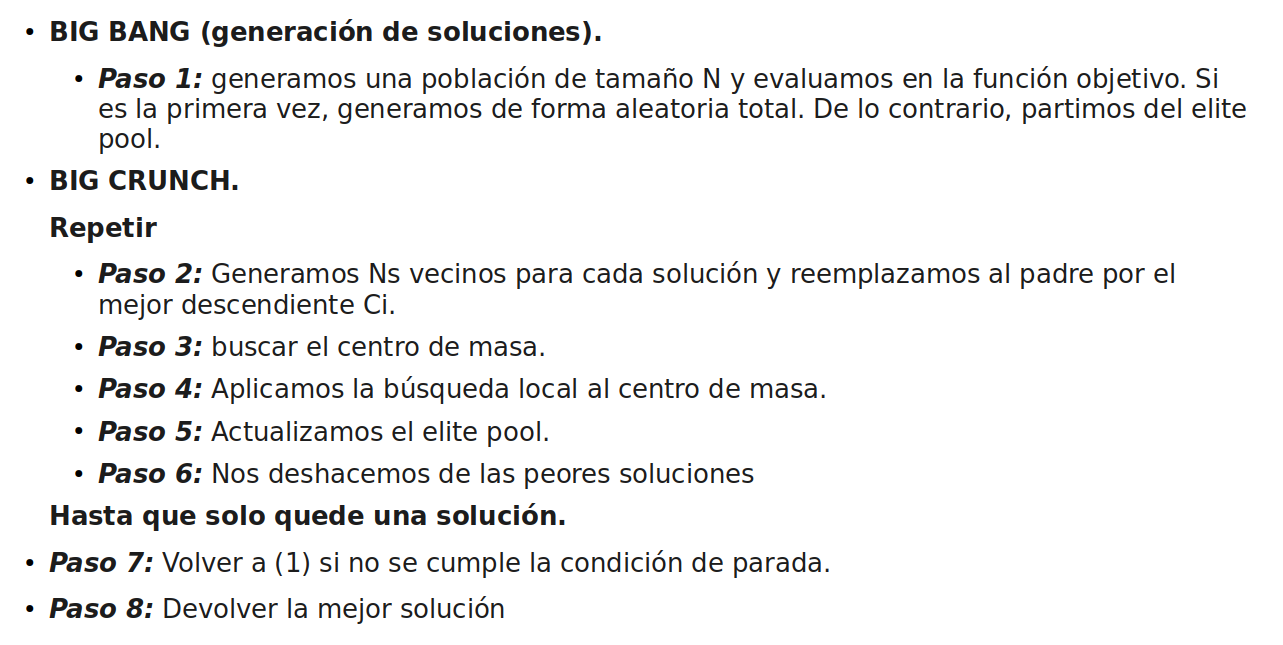
\includegraphics[scale=0.350]{Imagenes/pseudo.png}
\label{}
\end{figure}

\textbf{Mencionar que como en los criterios de evaluación del proyecto se evalúa por separado la metaheurística y una mejora de esta añadiéndole Búsqueda Local o cualquier otra hibridación, vamos a obviar el PASO 4 para la primera parte. Este paso lo añadiremos para la mejora. }

\subsubsection{Explicación de las partes del algoritmo}

\textbf{Paso 1:} nuestro algoritmo comienza con la fase del Big Bang, donde generamos nuestras soluciones inciales. En esta primera generación, dichas soluciones se generarán de manera totalmente aleatorias. Por el contrario, para el resto de generaciones de soluciones iniciales, partiremos del conjunto de élite. Luego cada vez se generarán poblaciones mejores. 

\begin{itemize}
\item \textbf{Conjunto de élite}: este es uno de los términos que mayor importancia cobra en el algoritmo. Este conjunto almacena aquellas soluciones que sean mejores. Esto, nos permite realizar una mayor explotación de las soluciones.  
\end{itemize}

Puesto que para la segunda práctica, para los algoritmos genéticos usamos poblaciones con tamaño 30, vamos a mantener el mismo tamaño de tal manera que podamos realizar una comparación coherente entre los algoritmos ya realizados. 

\textbf{Paso 2: } una vez realizada la fase del Big Bang, pasamos a la fase del Big Crunch. Lo primero que haremos en esta sección es que para cada solución actual generaremos $N_s$ vecinos, de tal manera que reemplazaremos al padre por el mejor descendiente $C_i$. 

En el BB-BC original la generación de vecinos se rige por las siguientes dos fórmulas: 
\begin{equation}
C_i^{new} = C_c + \sigma
\end{equation}
\begin{equation}
\sigma = \frac{r\alpha(C_{max} - C{min}}{k}, 0 < \frac{\alpha}{k} < 1
\end{equation}

donde $C_i^{new}$ es el vecino nuevo y $\sigma$ la desviación estándar de una distribución normal. 

Para el cálculo de $\sigma$, $r$ es un nº aleatorio entre el 0 y 1. Así mismo, $\alpha$ es una tasa de reducción cuyo valor también estará comprendido en dicho intervalo. $C_{max} y C_{min}$ son los límites superior e inferior del conjunto de élite en un momento dado. Por último, $k$ es el nº máximo de evaluaciones. 

En este paso es donde más adapto la metaheurística a nuestro problema. Como lo que queremos es modificar un vector de pesos, tenemos que darle otro sentido a la ecuación (1). Entonces, $\sigma$ significará para nosotros el porcentaje de pesos que vamos a mutar. De tal manera que, como mediante (2) se obtienen valores muy pequeños he procedido de la siguiente forma: 

\begin{equation}
\sigma = max\hspace{0.02cm}\{\hspace{0.02cm}C_{max} - C_{min}, 0.05\hspace{0.02cm}\}
\end{equation}

Sabemos que al principio el conjunto de élite tendrá soluciones con valores de masas más dispersos. Esto nos permite entonces, mutar una mayor cantidad de pesos al principio del algoritmo pues la diferencia entre $C_{max}$ y $C_{min}$ será bastante mayor que 0.05. Por el contrario, conforme avance la ejecución dicha diferencia irá reduciéndose. Cada vez se irán mutando menos pesos. Seguramente, llegue un punto en que sea muy pequeña, entonces nos aseguramos de que al menos se mutarán un 5\% de los pesos, de ahí que incluyamos el 0.05 en la ecuación (3). 

\textbf{Paso 3: }Tras esto, buscaremos el centro de masas: 

\begin{itemize}
\item \textbf{Centro de masas:} en física, el centro de masas de un sistema discreto o continuo es el punto geométrico que dinámicamente se comporta como si en él estuviera aplicada la resultante de las fuerzas externas al sistema. De manera análoga, se puede decir que el sistema formado por toda la masa concentrada en el centro de masas es un sistema equivalente al original.
\end{itemize}

En nuestro caso, el centro de masas hara referencia a aquella solución que mayor masa tenga, o lo que es lo mismo, aquella solución que mejor valor tenga para nuestra función objetivo. 

\textbf{Llegados a este punto es donde se aplicaría el paso 4 del algoritmo. Aplicaríamos una búsqueda local, con un determinado nº de evaluaciones máximas. Este paso solo se incluye en la hibridación con BL.}

\textbf{Paso 5: } la siguiente tarea a realizar es la de actualizar el \textbf{elite pool}. Para ello, borramos el último elemento del array (nótese que dicho vector de Stellar Objects ha sido ordenado previamente de forma descendente, de mayor a menor, en función de los valores de las masas). Acto seguido, incluiríamos el nuevo centro de masa, y procederíamos a realizar una ordenación de nuevo. Así mismo, almacenaríamos los nuevos valores de $c_{max}$ y $c_{min}$. 

\textbf{Paso 6: } una vez realizadas todas las operaciones necesarias para actualizar la elite pool, procederíamos a reducir el tamaño de la población actual. En cada iteración reducimos en 6 el tamaño actual. En caso de haber únicamente 6 individuos, nos quedaríamos directamente con el mejor, y saldríamos del bucle interno. 

\textbf{Paso 7: } una vez fuera, en caso de no cumplirse la condición de parada, volveríamos al PASO 1 del algoritmo, donde se generaría una nueva población inicial a partir del conjunto de élite actual resultante. Este proceso se repetirá hasta que se llegue al número de evaluaciones máximas permitidas, que es nuestro criterio de parada. 

A continuación presentamos el pseudocódigo de una manera mucho más extensa y cercana al código. En primer lugar, incluyo el pseudocódigo de la función \textbf{neighbours}. Mediante este método generaamos todos los vecinos para cada solución de la población actual. Posteriormente, retornamos aquel vecino cuyo valor de masa sea el más alto. 

\vspace{1cm}

\begin{algorithm}
\caption{neighbours}\label{euclid}
\begin{algorithmic}[1]
\Procedure{neighbours}{st,data,classes, trainIndex, testIndex, cmax, cmin}

\State \emph{for i in} range(NUM\_NEIGHBOURS): 
\State \hspace{1cm}\emph{for i in} range(nº caracteristicas * m)
\State \hspace{1.5cm} index $\gets$ nº aleatorio entre [0, nº características -1]
\State \hspace{1.5cm}mute(st.w)
\State \hspace{1cm}new\_st $\gets$ StellarObject(data[trainIndex], classes[trainIndex], st.w)
\State \hspace{1cm}neighbours.append(new\_st)

\State
\State return vecino con mayor valor de masa

\EndProcedure
\end{algorithmic}
\end{algorithm}

\vspace{1cm}

Ahora, vamos con el pseudocódigo de la función principal del algoritmo. Tal y como se comentó previamente, el paso 4 (incluir la búsqueda local no se incluye en esta versión inicial. Se incluirá en la hibridación explicada posteriormente. 

\begin{algorithm}
\caption{BBBC}\label{euclid}
\begin{algorithmic}[1]
\Procedure{BBBC}{data,classes, trainIndex, testIndex}

\State population $\gets$ población inicial aleatoria
\State sort(population)

\State centre\_mass $\gets$ population[0]
\State elite\_pool $\gets$ population[\hspace{0.1cm}:\hspace{0.1cm}ELITE\_POOL\_SIZE]
\State $c_{max}, c_{min} \gets$ elite\_pool[0], elite\_pool[-1]

\State
\State it $\gets$ 0 
\BState \textbf{\emph{while}}
it < MAX\_EVALUACIONES :

\State seguir $\gets$ true
\State new\_tam $\gets$ 30
\State \textbf{\emph{while}} seguir == True
\State \hspace{1cm}index $\gets$ índice característica aleatoria

\State \hspace{1cm}\emph{Para cada elemento de la población}

\State \hspace{1.5cm}neighbour $\gets$ neighbours(population[i], data, classes, trainIndex, testIndex, cmax, cmin)
\State \hspace{1.5cm} new\_population.apppend(neighbour)

\State \hspace{1cm}\emph{endloop}

\State
\State \hspace{1cm}it $\gets$ += new\_tam * NUM\_NEIGHBOURS

\State \hspace{1cm}sort(new\_population)
\State \hspace{1cm}centre\_mass $\gets$ new\_population[0]
\State
\State \hspace{1cm}Actualizamos elite\_pool
\State \hspace{1cm}sort(elite\_pool)
\State \hspace{1cm}$c_{max}, c_{min} \gets$ elite\_pool[0].mass, elite\_pool[-1].mass
\State \hspace{1cm}new\_population $\gets$ reducimos la poblacion

\State \textbf{\emph{end while}}

\State 
\State \textbf{if} it < MAX\_EVALUACIONES  \textbf{then}
\State \hspace{0.5cm} population $\gets$ generamos nueva población a partir del elite\_pool

\BState{end while}

\State Entrenamos el modelo, predecimos y calculamos las tasas
\State \textbf{return} tasa clasificación, tasa reducción
\EndProcedure
\end{algorithmic}
\end{algorithm}





















\newpage
\section{Procedimiento considerado para desarrollar el proyecto}
Para desarrollar la práctica, he usado \textbf{Python} como lenguaje de programación, sin usar ningún framework de metaheurísticas.

Para poder ejecutar el código , hace falta tener instalado \emph{Numpy, Scipy} y \emph{Sklearn}. Este último es muy útil para la realización de prácticas de este estilo pues trae implementaciones de muchas funcionalidades básicas para \emph{Machine learning}.

El fichero que hay que ejecutar dentro de la carpeta es el fichero \emph{\textbf{main.py}}. Para ello, basta con escribir en la terminal:
\[
\textit{python main.py}
\]
Tras la ejecución, comenzará a ejecutar los algoritmos sobre los 3 ficheros de datos que tenemos, que se explicarán más adelante.

La lista de archivos que contiene la práctica son los siguientes:
\begin{itemize}
	\item \textbf{main.py}: fichero principal a ejecutar para la ejecución de nuestro programa.	
	\item \textbf{algorithms.py}: fichero en el que se encuentran los algoritmos de la P1, y algunas funciones auxiliares programadas para las prácticas.

\item \textbf{genetics.py}: fichero con los algoritmos genéticos implementados en las prácticas.
\item \textbf{memetics.py}: fichero con los algoritmos meméticos implementados en las prácticas.

\item \textcolor{ugrColor}{\textbf{bbbc.py}: fichero con la metaheurística Big Bang - Big Crunch, y su híbrido.}
 
	\item \textbf{graficas.ipynb}: notebook mediante el cual he generado las gráficas.  
	\item \textbf{Datasets}: carpeta en la que se encuentran los datasets almacenados.
	\item \textbf{Archivos\_CSV}: carpeta con los archivos CSV necesarios para agilizar el proceso de creación de las gráficas.
	
\end{itemize}
\newpage
\section{Experimentos y análisis de resultados}

\subsection{Resultados de cada algoritmo}

\textbf{Algoritmo Big Bang - Big Crunch}

\begin{table}[ht!]
\begin{tabular}{ccccc|cccc|cccc}
\centering
 & \multicolumn{4}{c}{\textit{Ionosphere}} & \multicolumn{4}{c}{\textit{Parkinson}} & \multicolumn{4}{c}{\textit{Spectf-Heart}} \\ \hline
\textbf{Nº} & \textbf{Clas} & \textbf{Red} & \textbf{Agr} & \textbf{T} & \textbf{Clas} & \textbf{Red} & \textbf{Agr} & \textbf{T} & \textbf{Clas} & \textbf{Red} & \textbf{Agr} & \textbf{T} \\ \hline
0&	 0.90 & 0.97 & 0.94 & 23.56071 & 	0.69 & 1.00 & 0.85 & 14.11411 & 0.94 & 0.86 & 0.90 & 21.43855 \\ 
1&	 0.83 & 0.97 & 0.90 & 21.53296 & 	0.77 & 1.00 & 0.88 & 13.87712 & 0.84 & 0.91 & 0.88 & 21.63166 \\ 
2&	 0.74 & 0.91 & 0.83 & 22.06799 & 	0.85 & 1.00 & 0.92 & 14.12460 & 0.76 & 0.89 & 0.82 & 23.87600 \\ 
3&	 0.96 & 0.91 & 0.93 & 22.12468 & 	0.67 & 1.00 & 0.83 & 14.63036 & 0.83 & 0.80 & 0.81 & 22.49936 \\ 
4&	 0.96 & 0.91 & 0.93 & 22.28493 & 	0.72 & 1.00 & 0.86 & 13.73606 & 0.97 & 0.84 & 0.91 & 22.39183 \\ 
\hline
Media&	 0.88 & 0.94 & 0.91 & 22.31425 &	0.74 & 1.00 & 0.87 & 14.09645 &		0.87 & 0.86 & 0.86 & 22.36760
 \\ Std&	 0.08 & 0.03 & 0.04 & 0.67254 &	0.06 & 0.00 & 0.03 & 0.30468	&	0.08 & 0.04 & 0.04 & 0.86021
 \\
\end{tabular}
\end{table}

\textbf{Algoritmo Big Bang - Big Crunch + Búsqueda Local}

\begin{table}[ht!]
\begin{tabular}{ccccc|cccc|cccc}
\centering
 & \multicolumn{4}{c}{\textit{Ionosphere}} & \multicolumn{4}{c}{\textit{Parkinson}} & \multicolumn{4}{c}{\textit{Spectf-Heart}} \\ \hline
\textbf{Nº} & \textbf{Clas} & \textbf{Red} & \textbf{Agr} & \textbf{T} & \textbf{Clas} & \textbf{Red} & \textbf{Agr} & \textbf{T} & \textbf{Clas} & \textbf{Red} & \textbf{Agr} & \textbf{T} \\ \hline
0&	 0.77 & 0.91 & 0.84 & 24.60504 & 	0.74 & 1.00 & 0.87 & 14.72751 & 1.00 & 0.84 & 0.92 & 21.76347 \\ 
1&	 0.83 & 1.00 & 0.91 & 22.65621 & 	0.85 & 1.00 & 0.92 & 14.56661 & 0.90 & 0.89 & 0.89 & 22.40183 \\ 
2&	 0.89 & 0.94 & 0.91 & 22.60146 & 	1.00 & 1.00 & 1.00 & 15.42183 & 0.76 & 0.95 & 0.86 & 23.22098 \\ 
3&	 0.99 & 1.00 & 0.99 & 22.02246 & 	0.72 & 1.00 & 0.86 & 14.05384 & 0.89 & 0.86 & 0.87 & 23.19769 \\ 
4&	 0.94 & 0.97 & 0.96 & 21.90966 & 	0.67 & 1.00 & 0.83 & 14.01068 & 0.99 & 0.89 & 0.94 & 22.95220 \\ 
\hline
Media&	 0.88 & 0.96 & 0.92 & 22.75897 &	0.79 & 1.00 & 0.90 & 14.55609 &		0.91 & 0.89 & 0.90 & 22.70724
 \\ Std&	 0.08 & 0.03 & 0.05 & 0.97027	& 0.12 & 0.00 & 0.06 & 0.51551	&	0.09 & 0.04 & 0.03 & 0.55650\\

\end{tabular}
\end{table}

\pagebreak
\subsection{Resumen Global - Tabla de Medias}
\begin{table}[h]
\begin{tabular}{ccccc|cccc|cccc}
\centering
 & \multicolumn{4}{c}{\textit{Ionosphere}} & \multicolumn{4}{c}{\textit{Parkinson}} & \multicolumn{4}{c}{\textit{Spectf-Heart}} \\ \hline
\textbf{Alg} & \textbf{Clas} & \textbf{Red} & \textbf{Agr} & \textbf{T} & \textbf{Clas} & \textbf{Red} & \textbf{Agr} & \textbf{T} & \textbf{Clas} & \textbf{Red} & \textbf{Agr} & \textbf{T} \\ \hline
BL & 0.89 & 0.85 & 0.87 & 2.22200	&0.77 & 0.88 & 0.83 & 0.84650	&	0.88 & 0.82 & 0.85 & 3.60924\\
AGG-BLX & 0.89 & 0.62 & 0.75 & 18.27602	& 0.93 & 0.71 & 0.82 & 13.49899	&	0.85 & 0.58 & 0.72 & 20.67197 \\
AGG-AC & 0.91 & 0.66 & 0.79 & 17.86634&	0.97 & 0.75 & 0.86 & 12.70768&		0.87 & 0.64 & 0.76 & 21.65144 \\ 
AGE-BLX & 0.90 & 0.63 & 0.76 & 20.74966	&0.92 & 0.70 & 0.81 & 16.56119	&	0.86 & 0.59 & 0.72 & 24.35267 \\
AGE-AC & 0.92 & 0.88 & 0.90 & 20.62200&	0.98 & 0.94 & 0.96 & 15.86924	&	0.89 & 0.79 & 0.84 & 23.34907 \\
AM1 & 0.92 & 0.84 & 0.88 & 19.39848	&0.95 & 0.90 & 0.92 & 14.27740	&	0.88 & 0.80 & 0.84 & 21.06626 \\
AM2 & 0.90 & 0.71 & 0.80 & 19.68916	&0.94 & 0.72 & 0.83 & 12.72460	&	0.86 & 0.68 & 0.77 & 20.27860 \\
AM3 & 0.91 & 0.77 & 0.84 & 22.03035	&0.95 & 0.83 & 0.89 & 13.35908	&	0.88 & 0.73 & 0.80 & 20.43009 \\
\hline
BB-BC & 0.88 & 0.94 & 0.91 & 22.31425 &	0.74 & 1.00 & 0.87 & 14.09645 &		0.87 & 0.86 & 0.86 & 22.36760\\
BB-BC + LS & 0.88 & 0.96 & 0.92 & 22.75897 &	0.79 & 1.00 & 0.90 & 14.55609 &		0.91 & 0.89 & 0.90 & 22.70724
\end{tabular}
\end{table}


\subsection{Análisis de los resultados}

En esta sección realizaremos un extenso análisis a cerca de los resultados obtenidos. Para ello analizaremos cada una de las tasas. Empezamos en primer lugar por el tiempo de ejecución. 

\begin{tcolorbox}
\textbf{Primero, mencionar que para un mejor análisis visual recomiendo acudir al archivo .ipynb. Puesto que Plotly es una librería que permite la realización de gráficos interactivos, se pueden estudiar mucho mejor las comparativas. A continuación incluyo mis conclusiones tras examinar las distintas gráficas.}
\end{tcolorbox}

\subsubsection{Tiempo de ejecución}



\end{document}